\documentclass[12pt,a4paper]{article}

% ─── Page Layout ───────────────────────────────────────────────────────────────
\usepackage[a4paper, margin=0.8in, headheight=14pt]{geometry}

% ─── Fonts (XeLaTeX) ───────────────────────────────────────────────────────────
\usepackage{fontspec}
\usepackage{unicode-math}
\setmainfont{TeX Gyre Pagella}
\setmonofont[Scale=0.88]{TeX Gyre Cursor}
\setmathfont{Latin Modern Math}

% ─── Packages ──────────────────────────────────────────────────────────────────
\usepackage{xcolor}
\usepackage{colortbl}
\usepackage{titlesec}
\usepackage{enumitem}
\usepackage{tabularx}
\usepackage{booktabs}
\usepackage{array}
\usepackage{amsmath}
\usepackage{tikz}
\usetikzlibrary{shapes.geometric, arrows.meta, positioning, calc, fit, decorations.pathreplacing}
\usepackage{tcolorbox}
\tcbuselibrary{skins, breakable}
\usepackage{hyperref}
\usepackage{fancyhdr}
\usepackage{graphicx}
\usepackage{microtype}
\hyphenpenalty=10000
\exhyphenpenalty=10000
\sloppy
\usepackage{caption}
\usepackage{setspace}
\usepackage{multirow}
\usepackage{tocloft}

% ─── Q&A helper ────────────────────────────────────────────────────────────────
\newcommand{\Q}[1]{\textbf{#1}\par\noindent\ignorespaces}

% ─── Colour Palette ────────────────────────────────────────────────────────────
\definecolor{myred}{RGB}{196,30,58}
\definecolor{mydark}{RGB}{30,30,50}
\definecolor{mygreen}{RGB}{14,120,80}
\definecolor{myteal}{RGB}{0,130,140}
\definecolor{myamber}{RGB}{180,100,0}
\definecolor{mypurple}{RGB}{100,30,160}
\definecolor{mygray}{RGB}{246,247,249}
\definecolor{mgframe}{RGB}{180,185,200}
\definecolor{watermark}{RGB}{145,150,170}
\definecolor{hdrred}{RGB}{250,232,235}
\definecolor{hdrgreen}{RGB}{220,244,233}
\definecolor{hdrteal}{RGB}{220,242,244}
\definecolor{hdramber}{RGB}{253,242,215}
\definecolor{hdrpurple}{RGB}{238,228,255}
\definecolor{hdrgray}{RGB}{238,240,245}
\definecolor{rowalt}{RGB}{250,251,253}

% ─── Section Formatting ────────────────────────────────────────────────────────
\titleformat{\section}
  {\large\bfseries\color{myred}}{\thesection.}{0.5em}{}
  [\vspace{1pt}{\color{myred}\rule{\linewidth}{0.8pt}}]
\titleformat{\subsection}
  {\normalsize\bfseries\color{myteal}}{\thesubsection}{0.5em}{}
\titlespacing*{\section}{0pt}{18pt}{7pt}
\titlespacing*{\subsection}{0pt}{11pt}{4pt}

% ─── Paragraph ─────────────────────────────────────────────────────────────────
\setlength{\parindent}{0pt}
\setlength{\parskip}{4pt}

% ─── TOC Styling ───────────────────────────────────────────────────────────────
\renewcommand{\cfttoctitlefont}{\large\bfseries\color{myred}}
\renewcommand{\cftaftertoctitle}{\par\noindent{\color{myred}\rule{\linewidth}{0.8pt}}}
\setlength{\cftbeforetoctitleskip}{0pt}
\setlength{\cftaftertoctitleskip}{6pt}
\renewcommand{\cftsecfont}{\normalsize\bfseries\color{mydark}}
\renewcommand{\cftsecpagefont}{\normalsize\bfseries\color{mydark}}
\renewcommand{\cftsecleader}{\cftdotfill{\cftdotsep}}
\setlength{\cftbeforesecskip}{7pt}
\renewcommand{\cftsubsecfont}{\small\color{mydark}}
\renewcommand{\cftsubsecpagefont}{\small\color{mydark}}
\setlength{\cftbeforesubsecskip}{3pt}
\setlength{\cftsubsecindent}{1.4em}

% ─── Table helpers ─────────────────────────────────────────────────────────────
\renewcommand{\arraystretch}{1.45}
\setlength{\tabcolsep}{6pt}
\arrayrulecolor{mydark}
\newcolumntype{B}[1]{>{\small\bfseries\raggedright\arraybackslash}m{#1}}
\newcolumntype{Y}{>{\small\raggedright\arraybackslash}X}
\renewcommand{\tabularxcolumn}[1]{m{#1}}

% ─── Header / Footer ───────────────────────────────────────────────────────────
\pagestyle{fancy}
\fancyhf{}
\fancyhead[L]{\small\color{myred}\textbf{OE-EC604B}\;\color{mydark}--- Operating System}
\fancyhead[R]{\small\color{myteal}\textbf{Module 9 Notes}}
\fancyfoot[C]{\small\color{mydark}\thepage}
\fancyfoot[R]{\small\color{watermark}\textit{\copyright\ Biraj}}
\renewcommand{\headrulewidth}{0.5pt}
\renewcommand{\footrulewidth}{0.3pt}

% ─── Hyperref ──────────────────────────────────────────────────────────────────
\hypersetup{
  colorlinks=true, linkcolor=myteal, urlcolor=myteal,
  pdfauthor={Biraj Sarkar},
  pdftitle={OE-EC604B --- Module 9 Notes}
}

% ─── tcolorbox styles ──────────────────────────────────────────────────────────
\tcbset{
  tikzbox/.style={
    colback=mygray, colframe=mgframe, boxrule=0.6pt, arc=4pt,
    left=8pt, right=8pt, top=6pt, bottom=6pt,
    colbacktitle=mgframe, coltitle=mydark,
    fonttitle=\small\bfseries
  },
  defbox/.style={
    colback=hdrgreen, colframe=mygreen, boxrule=0.8pt, arc=4pt,
    left=9pt, right=9pt, top=6pt, bottom=6pt,
    colbacktitle=mygreen, coltitle=white,
    fonttitle=\small\bfseries
  },
  formulabox/.style={
    colback=hdrteal, colframe=myteal, boxrule=0.8pt, arc=4pt,
    left=9pt, right=9pt, top=7pt, bottom=7pt,
    colbacktitle=myteal, coltitle=white,
    fonttitle=\small\bfseries
  },
  examplebox/.style={
    colback=hdramber, colframe=myamber, boxrule=0.8pt, arc=4pt,
    left=9pt, right=9pt, top=6pt, bottom=6pt,
    colbacktitle=myamber, coltitle=white,
    fonttitle=\small\bfseries
  },
  masonbox/.style={
    colback=hdrpurple, colframe=mypurple, boxrule=0.8pt, arc=4pt,
    left=9pt, right=9pt, top=6pt, bottom=6pt,
    colbacktitle=mypurple, coltitle=white,
    fonttitle=\small\bfseries
  },
  exambox/.style={
    colback=hdrpurple, colframe=mypurple, boxrule=1pt, arc=5pt,
    left=10pt, right=10pt, top=8pt, bottom=8pt,
    colbacktitle=mypurple, coltitle=white,
    fonttitle=\bfseries,
    breakable, title after break={\textbf{Frequently Asked / Viva Questions (contd.)}}}
}
% Make all boxes breakable across pages
\tcbset{breakable}

% ─── TikZ styles ───────────────────────────────────────────────────────────────
\tikzset{
  block/.style={rectangle, draw=myteal, fill=hdrteal,
    text width=2.4cm, align=center, minimum height=0.95cm,
    font=\small, rounded corners=3pt, line width=0.7pt},
  redblock/.style={rectangle, draw=myred, fill=hdrred,
    text width=2.4cm, align=center, minimum height=0.95cm,
    font=\small, rounded corners=3pt, line width=0.7pt},
  greenblock/.style={rectangle, draw=mygreen, fill=hdrgreen,
    text width=2.4cm, align=center, minimum height=0.95cm,
    font=\small, rounded corners=3pt, line width=0.7pt},
  amberblock/.style={rectangle, draw=myamber, fill=hdramber,
    text width=2.4cm, align=center, minimum height=0.95cm,
    font=\small, rounded corners=3pt, line width=0.7pt},
  purpblock/.style={rectangle, draw=mypurple, fill=hdrpurple,
    text width=2.4cm, align=center, minimum height=0.95cm,
    font=\small, rounded corners=3pt, line width=0.7pt},
  sumjunc/.style={circle, draw=myamber, fill=hdramber,
    minimum size=0.62cm, font=\small, line width=0.8pt},
  arrow/.style={-Stealth, thick, color=mydark},
  redarrow/.style={-Stealth, thick, color=myred},
  line/.style={thick, color=mydark}
}

% ═══════════════════════════════════════════════════════════════════════════════
\begin{document}
% ═══════════════════════════════════════════════════════════════════════════════

\begin{center}
  {\LARGE\bfseries\color{myred} OE-EC604B --- Operating System}\\[5pt]
  {\normalsize\color{mydark} Semester VI \quad$\bullet$\quad 3L:0T:0P \quad$\bullet$\quad 3 Credits}\\[3pt]
  {\normalsize\color{myteal}\textbf{Module 9 Exam Notes: Protection, Security, and UNIX Case Study}}\\[3pt]
  {\small\color{mydark} CGEC \;$|$\; B.Tech ECE (2023--27) \;$|$\; \textit{Biraj Sarkar}}
\end{center}
\vspace{2pt}
\noindent{\color{myred}\rule{\linewidth}{1.5pt}}
\vspace{2pt}

\hypersetup{linkcolor=mydark}
\tableofcontents
\hypersetup{linkcolor=myteal}
\newpage

% ===============================================================================
\section{Protection \& Security}
% ===============================================================================

Modern computer systems must protect data from unauthorized access, modification, and destruction.
\begin{itemize}[leftmargin=*, itemsep=3pt]
  \item \textbf{Protection:} A mechanism for controlling the access of programs, processes, or users to the resources defined by a computer system.
  \item \textbf{Security:} A measure of confidence that the integrity of a system and its data will be preserved against external threats (viruses, hackers, physical damage).
\end{itemize}

\subsection{Access Matrix Model}
The \textbf{Access Matrix} is a formal protection model. It views the system as a set of \textbf{domains} (active entities, e.g., users, processes) and \textbf{objects} (passive hardware/software components, e.g., files, printers).
\begin{itemize}[leftmargin=*, itemsep=3pt]
  \item \textbf{Grid Entry:} $\text{Matrix}[D, O]$ defines the access rights (read, write, execute) that process in domain $D$ has over object $O$.
  \item \textbf{Implementations:}
  \begin{itemize}[leftmargin=*, itemsep=2.5pt, topsep=0pt]
    \item \textbf{Access Control List (ACL):} Associates with each object a list of domains and their permitted rights (columns of the matrix). Used in Unix/Windows filesystems.
    \item \textbf{Capability List (C-List):} Associates with each domain a list of objects and rights (rows of the matrix).
    \end{itemize}
  \end{itemize}

% ===============================================================================
\section{Introduction to Distributed Operating Systems}
% ===============================================================================

A \textbf{Distributed Operating System} manages a collection of independent, networked, and physically separate computational nodes, presenting them to the user as a single, unified computer system.
\begin{itemize}[leftmargin=*, itemsep=3pt]
  \item \textbf{Network OS vs. Distributed OS:} In a Network OS, users are aware of the existence of multiple computers (e.g., must use \texttt{ssh} or remote mounting). A Distributed OS provides \textbf{location transparency} --- the user cannot tell where a program is running or where a file is stored.
\end{itemize}

% ===============================================================================
\section{Case Study: The UNIX Operating System}
% ===============================================================================

UNIX is a highly modular, multitasking operating system originally developed at Bell Labs.

\subsection{System Architecture}
UNIX is divided into three main layers:
1. \textbf{User Space:} Applications, library calls, and the command interpreter (Shell).
2. \textbf{Kernel Space:} Manages process execution, memory, file systems, interrupts, and I/O.
3. \textbf{Hardware:} The underlying CPU, memory, and physical controllers.

\subsection{The UNIX File System (Inode Structure)}
In UNIX, every file is represented by a data structure called an \textbf{Inode (Index Node)}. The inode contains file metadata (owner, permissions, size, time stamps) and a table of \textbf{block addresses} pointing to the physical data on disk.

\begin{itemize}[leftmargin=*, itemsep=3pt]
  \item \textbf{Inode Address Pointers Layout:} Typically contains 15 pointers:
  \begin{itemize}[leftmargin=*, itemsep=2.5pt, topsep=0pt]
    \item \textbf{Pointers 0–11:} \textbf{Direct Blocks} (point directly to disk data blocks).
    \item \textbf{Pointer 12:} \textbf{Single Indirect Block} (points to a block containing pointers to data blocks).
    \item \textbf{Pointer 13:} \textbf{Double Indirect Block} (points to a block containing pointers to single indirect blocks).
    \item \textbf{Pointer 14:} \textbf{Triple Indirect Block} (points to a block containing pointers to double indirect blocks).
    \end{itemize}
  \end{itemize}

\begin{tcolorbox}[tikzbox, title={UNIX Inode Block Mapping Architecture}]
\centering
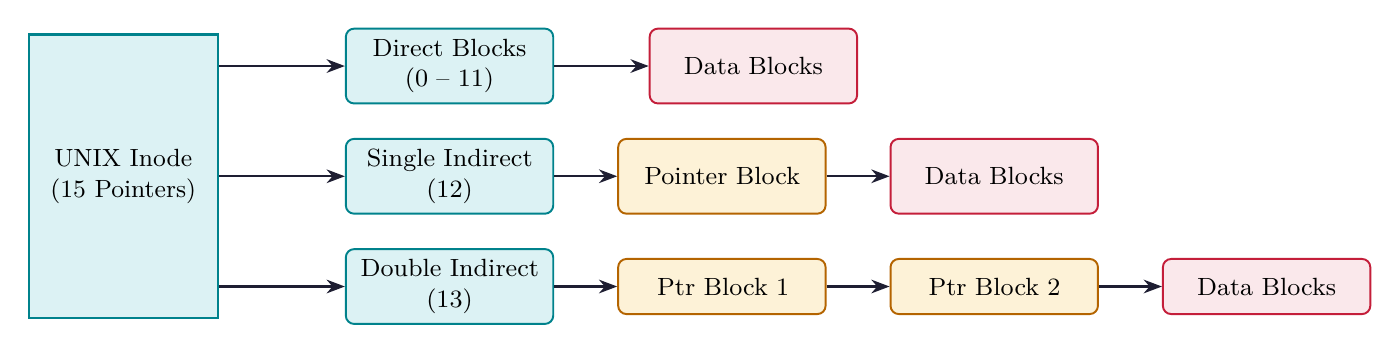
\begin{tikzpicture}[node distance=0.6cm and 1.8cm, thick, font=\small]
  % Inode
  \node[draw=myteal, fill=hdrteal, minimum width=2.4cm, minimum height=3.6cm, align=center] (inode) {UNIX Inode\\(15 Pointers)};
  
  % Direct Blocks
  \node[block, right=1.6cm of inode, yshift=1.4cm] (direct) {Direct Blocks\\(0 -- 11)};
  \node[block, right=1.2cm of direct, fill=hdrred, draw=myred] (db) {Data Blocks};
  
  % Single Indirect
  \node[block, right=1.6cm of inode, yshift=0.0cm] (ind1) {Single Indirect\\(12)};
  \node[block, right=0.8cm of ind1, fill=hdramber, draw=myamber] (pt1) {Pointer Block};
  \node[block, right=0.8cm of pt1, fill=hdrred, draw=myred] (db2) {Data Blocks};
  
  % Double Indirect
  \node[block, right=1.6cm of inode, yshift=-1.4cm] (ind2) {Double Indirect\\(13)};
  \node[block, right=0.8cm of ind2, fill=hdramber, draw=myamber, minimum height=0.7cm] (pt2) {Ptr Block 1};
  \node[block, right=0.8cm of pt2, fill=hdramber, draw=myamber, minimum height=0.7cm] (pt3) {Ptr Block 2};
  \node[block, right=0.8cm of pt3, fill=hdrred, draw=myred, minimum height=0.7cm] (db3) {Data Blocks};

  \draw[arrow] (inode.east |- direct.west) -- (direct.west);
  \draw[arrow] (direct.east) -- (db.west);
  
  \draw[arrow] (inode.east) -- (ind1.west);
  \draw[arrow] (ind1.east) -- (pt1.west);
  \draw[arrow] (pt1.east) -- (db2.west);
  
  \draw[arrow] (inode.east |- ind2.west) -- (ind2.west);
  \draw[arrow] (ind2.east) -- (pt2.west);
  \draw[arrow] (pt2.east) -- (pt3.west);
  \draw[arrow] (pt3.east) -- (db3.west);
\end{tikzpicture}
\end{tcolorbox}

\subsection{UNIX Process Management \& Scheduling}
\begin{itemize}[leftmargin=*, itemsep=3pt]
  \item \textbf{Process Creation:} Handled exclusively via \texttt{fork()} followed by \texttt{exec()}.
  \item \textbf{UNIX Process States:} Running in user mode, Running in kernel mode, Ready to run in memory, Asleep in memory (waiting for I/O), Ready to run swapped, Asleep swapped, Zombie (terminated but parent has not read exit status).
  \item \textbf{UNIX CPU Scheduling:} Uses a multilevel feedback queue scheduling algorithm. Priority is recalculated every second based on CPU usage:
\end{itemize}
$$\text{Priority} = \text{Base} + \frac{\text{Recent CPU Usage}}{2} + \text{Nice}$$
where \texttt{Nice} is a user-controllable process parameter (higher \texttt{Nice} value lowers priority).

\newpage
% ===============================================================================
% MANDATORY QUICK REVISION PAGE
% ===============================================================================
\begin{center}
  {\large\bfseries\color{myred} Quick Revision --- Module 9}\\[3pt]
  {\small\color{mydark} Protection, Security and UNIX Case Study $|$ OE-EC604B}
\end{center}
\noindent{\color{myred}\rule{\linewidth}{1.2pt}}
\vspace{4pt}

\begin{tcolorbox}[formulabox, title={\textbf{UNIX Inode Max File Size Calculations}}]
Let block size = $1\,\text{KB}$. Disk address pointer = $4\,\text{Bytes}$.
\begin{itemize}[leftmargin=*, itemsep=3pt]
  \item \textbf{Max Direct Blocks Capacity:} $12 \times 1\,\text{KB} = 12\,\text{KB}$.
  \item \textbf{Max Single Indirect Capacity:} $(1\,\text{KB} / 4\,\text{B}) \times 1\,\text{KB} = 256 \times 1\,\text{KB} = 256\,\text{KB}$.
  \item \textbf{Max Double Indirect Capacity:} $256 \times 256 \times 1\,\text{KB} = 64\,\text{MB}$.
  \item \textbf{Max Triple Indirect Capacity:} $256 \times 256 \times 256 \times 1\,\text{KB} = 16\,\text{GB}$.
  \item \textbf{Total Max File Size Limit:} $12\,\text{KB} + 256\,\text{KB} + 64\,\text{MB} + 16\,\text{GB} \approx 16.06\,\text{GB}$.
\end{itemize}
\end{tcolorbox}

\begin{tcolorbox}[defbox, title={\textbf{One-Line Definitions}}]
\begin{itemize}[leftmargin=*, itemsep=2.5pt, topsep=0pt]
  \item \textbf{Access Matrix:} Grid model representing domains (rows), objects (columns), and access rights (cells).
  \item \textbf{ACL:} Access Control List; column-wise access matrix stored on objects indicating permitted domains.
  \item \textbf{Capability List:} Row-wise access matrix stored inside process domains detailing object rights.
  \item \textbf{Distributed OS:} OS presenting multiple physical CPU nodes as a single logical computer transparently.
  \item \textbf{Location Transparency:} File or computation access method independent of physical node location.
  \item \textbf{Superblock:} UNIX filesystem metadata block containing system size, free block count, and inode limits.
  \item \textbf{UNIX Inode:} Index block detailing metadata and 15 storage pointers for a UNIX file.
  \item \textbf{Zombie Process:} Process that has terminated but still occupies an entry in the process table.
\end{itemize}
\end{tcolorbox}

\begin{tcolorbox}[exambox, title={\textbf{Frequently Asked / Viva Questions}}]
\begin{enumerate}[topsep=0pt, label=\textbf{Q\arabic*.}, itemsep=5pt]
  \item \Q{Differentiate between Protection and Security in operating systems.}
    Protection is the internal OS mechanism to control process/user access to defined system resources. Security is the external defense mechanism protecting system integrity and data against threats like malware, hackers, and environment disasters.
  \item \Q{Compare Access Control Lists (ACLs) and Capability Lists (C-Lists).}
    ACLs are column-oriented implementations of the Access Matrix; they associate permitted domains and rights directly with each object (e.g., file permissions). C-Lists are row-oriented; they attach object rights to each domain/user process directly.
  \item \Q{What is a Distributed Operating System? What are its primary advantages?}
    A Distributed OS coordinates multiple autonomous CPUs connected by communication networks, presenting them as a single logical machine. Advantages include resource sharing, computational speedup, reliability (fault tolerance), and scalability.
  \item \Q{Explain the UNIX Inode pointer layout and calculate max file size for a 2 KB block size with 4-byte pointers.}
    Layout has 12 direct, 1 single indirect, 1 double indirect, and 1 triple indirect pointers.
    \textbf{Pointers per block} = $2\,\text{KB} / 4\,\text{B} = 512$.\par
    \textbf{Direct size} = $12 \times 2\,\text{KB} = 24\,\text{KB}$.\par
    \textbf{Single indirect size} = $512 \times 2\,\text{KB} = 1024\,\text{KB} = 1\,\text{MB}$.\par
    \textbf{Double indirect size} = $512^2 \times 2\,\text{KB} = 512\,\text{MB}$.\par
    \textbf{Triple indirect size} = $512^3 \times 2\,\text{KB} = 256\,\text{GB}$.\par
    \textbf{Max File Size} = $24\,\text{KB} + 1\,\text{MB} + 512\,\text{MB} + 256\,\text{GB} \approx 256.5\,\text{GB}$.
  \item \Q{What is the function of the Superblock in the UNIX file system?}
    The Superblock is located at a fixed offset near the start of the disk partition. It contains critical metadata about the file system, including total blocks, free block count, free inode list, size of inode list, and status flag.
  \item \Q{Describe the UNIX process scheduling formula and explain the role of the nice value.}
    $\text{Priority} = \text{Base} + (\text{Recent CPU Usage} / 2) + \text{Nice}$. The OS decays priority based on CPU usage to prevent CPU starvation. The \texttt{Nice} value is an administrator/user offset (ranging from $-20$ to $+19$). A higher nice value increases the priority value, which actually lowers scheduling priority.
  \item \Q{What is a zombie process in UNIX? How is it cleared?}
    A zombie process is a process that has finished execution but still has an entry in the system process table to allow its parent to read its exit code (via \texttt{wait()}). It is cleared when the parent executes a \texttt{wait()} system call. If the parent terminates, the zombie is inherited by the \texttt{init} process, which automatically calls \texttt{wait()}.
  \item \Q{Differentiate between Loosely Coupled and Tightly Coupled distributed systems.}
    Loosely coupled systems have independent nodes with private memory connected via slow communication networks (e.g., LAN clusters). Tightly coupled systems share a common physical memory and bus architecture with fast inter-processor communication.
  \item \Q{What is the Access Matrix model? How is it represented?}
    It is a security model where rows represent domains, columns represent objects, and cell entries represent the set of access rights (read, write, execute) allowed for a domain over an object.
  \item \Q{Explain the role of the shell in the UNIX operating system.}
    The shell is a user-space application that acts as a command line interpreter, reading user commands, expanding wildcards, setting up I/O redirection/piping, and spawning processes using \texttt{fork}/\texttt{exec} to execute those commands.
\end{enumerate}
\end{tcolorbox}

\begin{tcolorbox}[tikzbox, title={Security Implementation Comparison}]
\renewcommand{\arraystretch}{1.4}
\par\noindent
\begin{tabularx}{\linewidth}{|B{2.2cm}|>{\small\centering\arraybackslash}X|>{\small\centering\arraybackslash}X|}
\hline
\textbf{Feature} & \textbf{\color{myred}Access Control List (ACL)} & \textbf{\color{myteal}Capability List (C-List)} \\
\hline
\textbf{Association} & Attached to the Object (e.g. File) & Attached to the Subject (e.g. Domain) \\
\hline
\textbf{Revocation} & Easy (just delete domain from file list) & Hard (must search all domain lists) \\
\hline
\textbf{Access check} & Slow (must search file ACL at access) & Fast (domain presents token directly) \\
\hline
\textbf{Common use} & Standard OS filesystems & Object-oriented/microkernel systems \\
\hline
\end{tabularx}
\end{tcolorbox}

\end{document}
